\documentclass[12pt]{article}
\usepackage{fancyhdr}
\usepackage{datetime2}
\usepackage{amsmath}
\usepackage{amsfonts}
\usepackage{graphicx}
\usepackage{subcaption}
\usepackage[a4paper, left=1in, right=1in, bottom=1.25in]{geometry}

% set up headers and footers
\pagestyle{fancy}
\fancyhf{}
\lhead{Operating System Concepts Notes}
\rfoot{Page \thepage}
\setlength{\headheight}{15pt}

\begin{document}
\section*{OS Concepts 1.1: What Operating Systems Do}

\begin{itemize}
    \item \textbf{What is an OS?:} OS's vary widely in design and in function, but basically an OS is the software that sits between application programs and computer hardware. It provides an environment in which application programs are executed, by allocating physical resources like CPU, memory, and I/O devices.
\end{itemize}

\section*{OS Concepts 1.2: Computer-System Organization}

\subsection*{1.2.1: Interrupts}

\begin{itemize}
    \item \textbf{Device Controller:} The I/O managing processor within a device.
    \item \textbf{Device Driver:} A component in the OS that understands how to communicate with its respective device controller and manages I/O to those devices.
    \item \textbf{Interrupts:} Interrupts are used in OS's to handle asynchronous events originating from outside the processor (interrupts originating from within the processor are called exceptions). Device controllers and hardware faults raise interrupts. Because interrupts are used so heavily for time-sensitive processing, efficient interrupt handling is necessary for good system performance.
    \item \textbf{Interrupt Vector:} A table of pointers stored in low memory that holds the addresses of the interrupt service routines.
    \item \textbf{Basic Interrupt Implementation:} The CPU hardware has a wire called the interrupt-request line that the CPU senses after executing every instruction. When the CPU detects a device controller has asserted a signal on the wire, it reads the interrupt number and jumps to the respective interrupt-handler routine by using the interrupt number as an index into the interrupt vector. It then saves the current state of whatever was interrupted, and starts execution of the interrupt-handler routine. Once the handler is finished executing, it performs a state restore and returns the CPU to the execution state prior to the interrupt.
    \item \textbf{Interrupt Terminology:} We say that the device controller \textbf{raises} an interrupt by asserting a signal on the interrupt request line, the CPU \textbf{catches} the interrupt and \textbf{dispatches} it to the interrupt handler, and the handler \textbf{clears} the interrupt by servicing the device.
    \item \textbf{More Sophisticated Interrupt Implementation:} We need the ability for the following:
        \begin{itemize}
            \item Defer interrupt handling during critical processing
            \item Efficiently dispatch to the correct interrupt-handler for a device
            \item Multilevel interrupts, so that the OS can distinguish between high and low priority interrupts and respond with the appropriate level of urgency
        \end{itemize}

        To do this, most CPU's have two interrupt request lines: one is the nonmaskable interrupt, which is used for events such as unrecoverable memory errors, and the second is the maskable interrupt, which the CPU can turn off before the execution of critical instruction sequences that must not be interrupted. Device controllers use the maskable interrupt to request service.
\end{itemize}

\subsection*{1.2.2: Storage Structure}

\begin{itemize}
    \item \textbf{Firmware:} Software stored in ROM or EEPROM for booting the system and managing low level hardware.
\end{itemize}

\subsection*{1.2.3: I/O Structure}

\begin{itemize}
    \item \textbf{Direct Memory Access (DMA):} Interrupt-driven I/O as described in section 1.2.1 is fine for moving small amounts of data but can produce high overhead when used for bulk data movement, like when moving data to and from nonvolatile memory. DMA is used to avoid this overhead. The device controller sets up buffers, pointers, and counters for its I/O device, and transfers entire blocks of data to or from the device and main memory, with no intervention by the CPU. Only one interrupt is generated per block, to tell the device driver that the operation has completed, rather than the one interrupt per byte generated for low-speed devices. The CPU is able to perform other work while the device controller is performing these operations.
\end{itemize}

\section*{OS Concepts 1.3: Computer-System Architecture}

\subsection*{1.3.1: Single-Processor Systems}

\begin{itemize}
    \item \textbf{CPU:} The hardware that executes instructions.
    \item \textbf{Processor:} A physical chip that contains one or more CPU's.
    \item \textbf{CPU Core:} The core is the component of the CPU that executes instructions and contains registers for storing data locally.
    \item \textbf{Single-Processor System:} A computer system with a single processor containing one CPU with a single processing core. These systems often also have other special-purpose processors as well, such as disk, keyboard, and graphics controllers. These special-purpose processors run a limited instruction set and do not run processes; their use is incredibly common and does not turn a single-processor system into a multiprocessor system.
\end{itemize}

\subsection*{1.3.2: Multiprocessor Systems}

\begin{itemize}
    \item \textbf{Multiprocessor Systems:} A computer system containing multiple processors. Traditionally contains two or more processors, each with a single-core CPU.
        \begin{figure}[ht]
            \centering
            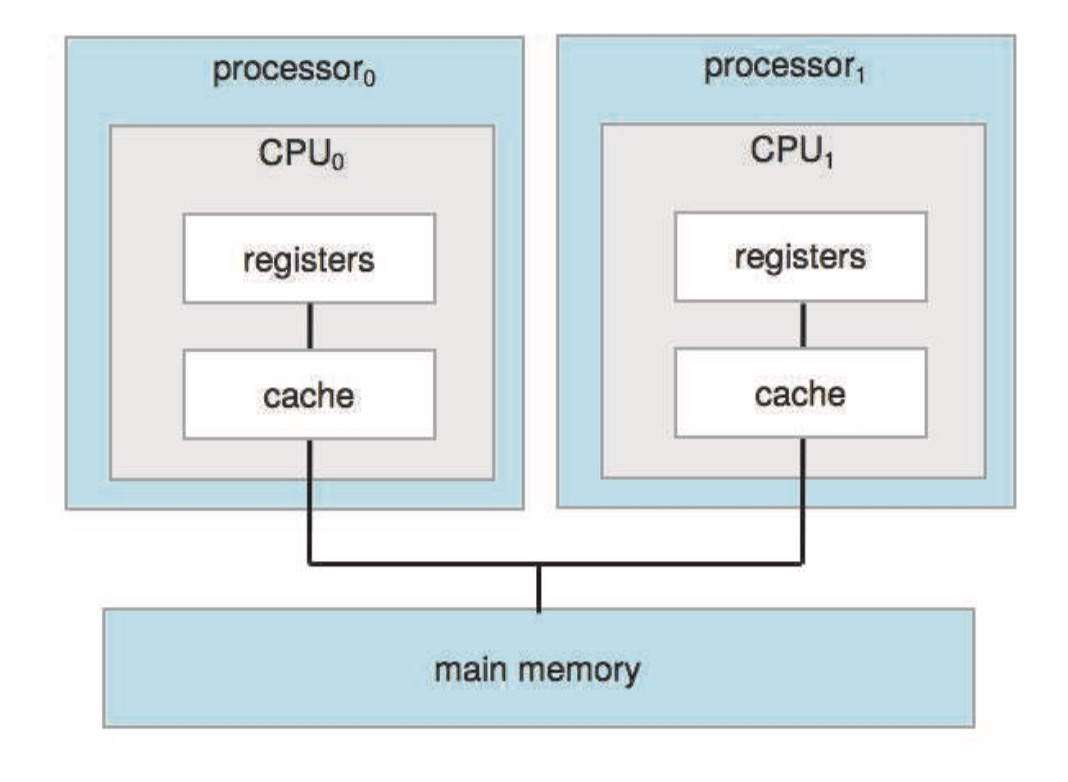
\includegraphics[width=0.6\textwidth]{figures/symmetric-multiprocessing-architecture.jpg}
            \caption{Symmetric \textit{multiprocessing} architecture}
            \label{fig:symmetric-multiprocessing-architecture}
        \end{figure}
    \item \textbf{Multiprocessor Advantages (Increased Throughput):} Primary advantages of multiprocessor systems is increased throughput. The speed-up ratio with \(N\) processors is not \(N\), however; it is less than \(N\) because there is overhead incurred and contention for shared resources when dealing with multiple processors.
    \item \textbf{Multicore Systems:} A computer system containing multiple cores on the same processor chip. Such systems can be more efficient than multiple chips with single cores because on-chip communication is faster than between-chip communication. Additionally, one chip with multiple cores uses significantly less power than multiple single-core chips, an issue especially important for mobile devices.
        \begin{figure}[ht]
            \centering
            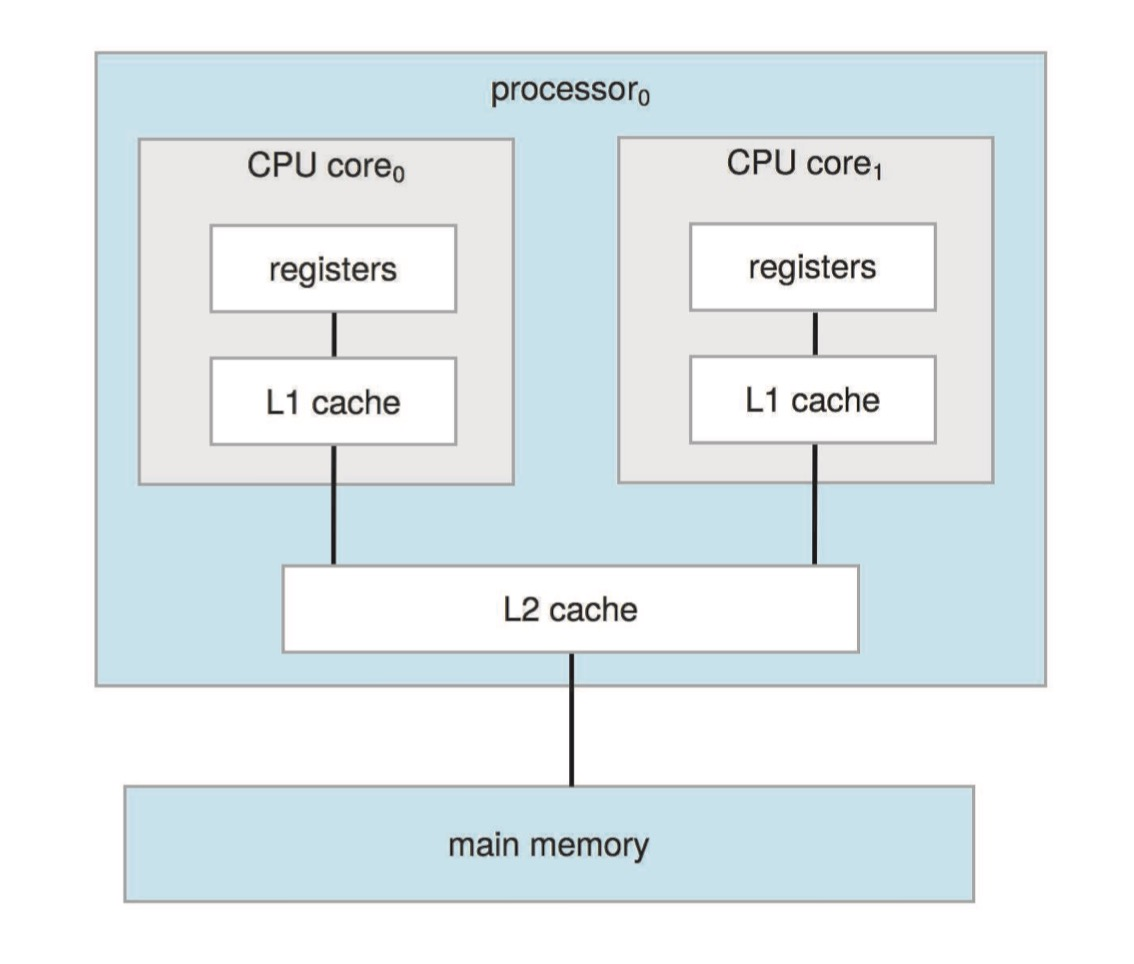
\includegraphics[width=0.6\textwidth]{figures/multicore-architecture.jpg}
            \caption{\textit{Multicore} architecture}
            \label{fig:multicore-architecture}
        \end{figure}
    \item \textbf{Multiprocessor Bottleneck:} Adding additional CPU's to a multiprocessor system increases computing power, but does not scale very well. Once too many CPU's are added, contention for the system bus becomes a bottleneck and performance begins to degrade.
    \item \textbf{Non-uniform Memory Access (NUMA):} To avoid bottleneck performance degradation arising from system bus contention, we can provide each CPU with its own local memory that is accessed via a small and fast local bus. The CPU's are connected by a shared system interconnect, so that all CPU's share one physical address space. The advantage is that when a CPU accesses its local memory, not only is it fast, but there is also no contention over the system interconnect. Thus, NUMA systems can scale more effectively as more processors are added.
        \begin{figure}[ht]
            \centering
            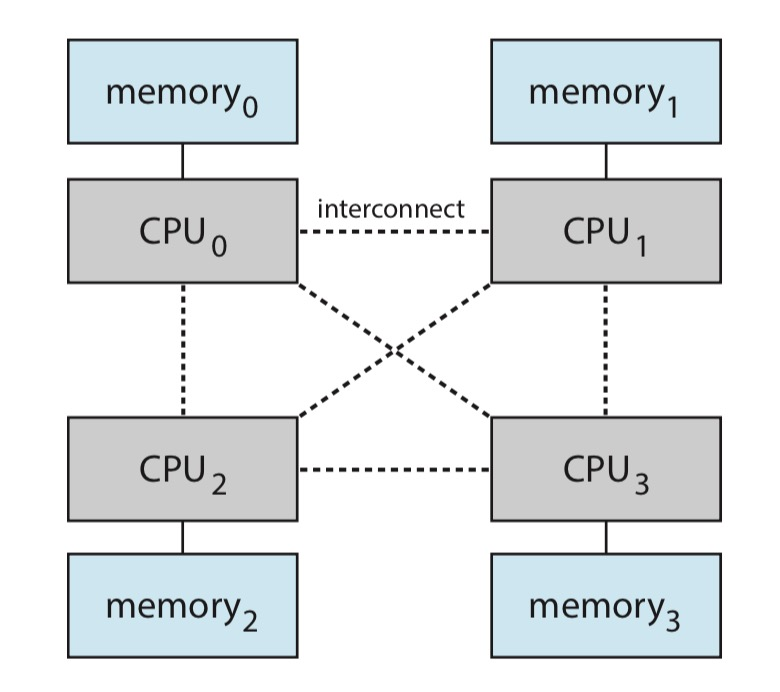
\includegraphics[width=0.4\textwidth]{figures/numa-architecture.jpg}
            \caption{NUMA architecture}
            \label{fig:numa-architecture}
        \end{figure}
    \item \textbf{NUMA Drawbacks (Increased Latency):} A potential drawback is increased latency when a CPU must access remote memory across the system interconnect (accessing the local memory of another CPU). OS's can minimize this NUMA penalty through careful CPU scheduling and memory management.
\end{itemize}

\section*{OS Concepts 1.4: Operating-System Operations}

\begin{itemize}
    \item \textbf{Bootstrap Program:} The initial program that is run when a computer starts running for the first time. Typically a very simple program and stored in firmware. The program must know how to load the OS kernel into memory and start executing it.
    \item \textbf{System Daemons:} Services provided outside of the kernel that are loaded into memory at boot time, which run the entire time the kernel is running.
\end{itemize}

\subsection*{1.4.1: Multiprogramming and Multitasking}

\begin{itemize}
    \item \textbf{Multiprogramming:} Increase CPU utilization by organizing programs so that the CPU always has one to execute. Execute a process until it needs to wait on some task like I/O, then switch to another process. Keep switching between processes such that the CPU is never idle.
    \item \textbf{Process:} In a multiprogrammed system, a program in execution is termed a process.
    \item \textbf{Multitasking:} The logical extension of multiprogramming. In multitasking systems, the CPU executes multiple processes by switching among them incredibly frequently. This is how interactive I/O like keyboard input works: rather than letting the CPU sit idle in the time between the keystrokes of the user, the OS will rapidly switch to another process in the meantime.
\end{itemize}

\subsection*{1.4.2: Dual-Mode and Multimode Operation}

\begin{itemize}
    \item \textbf{Modes of Execution:} A properly designed OS must ensure that an incorrect (or malicious) program cannot cause other programs - or the OS itself - to execute incorrectly. To do this, we need to distinguish between the execution of OS code and user-defined code. Most computer systems provide hardware support that allows differentiation among various modes of execution.
    \item \textbf{User Mode and Kernel Mode:} At the very least, we need two separate modes of operation: user mode and kernel mode (also called supervisor mode, system mode, or privileged mode). A bit, called the mode bit, is added to the hardware of the computer to indicate the current mode: kernel (0) or user (1). Whenever the OS gains control of the computer, it is in kernel mode. The system always switches back to user mode before passing control to a user program. The concept of modes can be extended beyond two modes (e.g. the four protection rings in Intel processors).
    \item \textbf{Privileged Instructions:} Some machine instructions that may cause can only be executed in kernel mode. The instruction to switch to kernel mode is an example of a privileged instruction.
\end{itemize}

\subsection*{1.4.3: Timer}

\begin{itemize}
    \item \textbf{Timer:} We must ensure that the OS maintains control over the CPU: we allow user programs to execute, but they must eventually relinquish control to the OS (avoid situations like user program infinite loops or not calling system services and thus not returning control to the OS). To accomplish this, we can use a timer that is set to raise an interrupt after a specified amount of time. If the timer interrupts, control transfers automatically to the OS, which may treat the interrupt as a fatal error or may give the program more time. Instructions that modify the timer are clearly privileged.
\end{itemize}

\section*{OS Concepts 1.5: Resource Management}

The OS can be seen as a resource manager. The following are things that the OS must carefully manage in a computer system.

\subsection*{1.5.1: Process Management}

\begin{itemize}
    \item \textbf{Program vs Process:} A program by itself is not a process. A program is a \textit{passive} entity, whereas a process is an \textit{active} entity. Remember that a process is just a program in execution, thus there can be multiple processes associated with the same program (and each is considered a separate execution sequence).
\end{itemize}

\subsection*{1.5.2: Memory Management}

\begin{itemize}
    \item \textbf{Memory Management:} The OS is responsible for keeping tack of which parts of memory are currently being used and which process is using them, allocating and deallocating memory, and deciding which processes (or parts of processes) and data to move into and out of memory.
\end{itemize}

\subsection*{1.5.3: File-System Management}

\begin{itemize}
    \item \textbf{File System:} The OS abstracts the physical properties of its storage devices to define a logical storage unit, the \textbf{file}. In other words, the OS implements the abstract concept of a file by managing mass storage media and the devices that control them.
\end{itemize}

\subsection*{1.5.4: Mass-Storage Management}

\begin{itemize}
    \item \textbf{Secondary Storage Management:} The proper management of secondary storage is critical to a computer system. The OS must take care of things such as mounting and unmounting, free-space management, storage allocation, disk scheduling, partitioning, and protection.
\end{itemize}

\subsection*{1.5.5: Cache Management}

\begin{itemize}
    \item \textbf{OS and Memory Hierarchy:} The OS is responsible for moving data between the different levels of the memory hierarchy that it has access to. The OS can only manipulate software-controlled caches, for instance transfer of data from disk to memory, while data transfer from CPU cache to registers is a hardware function.
    \item \textbf{Caches and Multitasking:} In a computing environment where only one process executes at a time, having the same data appear in multiple levels of the memory hierarchy is not an issue, since access to desired memory always will be to the copy at the highest level of the hierarchy. In a multitasking environment, however, extreme care must be taken to ensure that if several processes wish to access the same data, each of these processes obtains the most recently updated value of the data.
    \item \textbf{Caches and Multiprocessor Systems:} In a multiprocessing environment, not only do we need to make sure that processes access the most recenly updated value of the desired data (multitasking), but we now have CPUs that contain local caches in which data may esist simultaneously in several of these. We need to make sure that an update to the value of a given piece of data in one cache is immediately reflected in all other caches where this data resides. This issue if called \textit{cache conherency}, and is usually handled in hardware (below the OS level).
\end{itemize}

\subsection*{1.5.6: I/O System Management}

\begin{itemize}
    \item \textbf{I/O Subsystem:} One of the purposes of an OS is to hide the peculiarities of specific hardware devices from the user. Often, these peculiarities are hidden from most of the OS itself by the I/O subsystem. Device drivers for specific hardware devices for instance are included in the I/O subsystem.
\end{itemize}

% \vspace{4mm}

% \noindent Test here test

\end{document}
